%----------------------------------------------------------------------------
\chapter{Automatizált feladatkiértékelő modul}\label{chapter:exercise}
%----------------------------------------------------------------------------

A JPorta egyik fő funkciója a beadott feladatmegoldások automatikus kiértékelése. Ennek tervezése során törekedtek az általános, könnyen bővíthető megoldás megtalálására, amikkel akár nem programozási jellegű feladatokat is ki lehet adni. \cite{DudiMsc}

Az elkészült modul blokkokat használ alapvető építő elemeinek, melyek egy-egy kiértékelési feladatot valósítanak meg. Ennek köszönhetően új igény esetén nem kell a meglévő blokkokat módosítani, csak az új funkciót megvalósító blokkot implementálni.

A blokkok közötti kommunikációt bemeneti és kimeneti csatlakozóik teszik lehetővé. Ezek szabadon összeköthetőek bármely más blokk ellenkező típusú csatlakozójával, pl. a felhasználói fájl blokk kimenetét ráköthetjük a GCC fordító blokk bemenetére, így lefordíhatjuk az adott forrásfájlt (rendelkezésre álló blokkok pontos leírását ld. \ref{table:blocks}). Ezen kívül lehetnek olyan paraméterei is egy blokknak, melyeket adminisztrátori felületen kell beállítani, pl. fordítás esetén a fordítónak átadott kapcsolók.

\begin{table}[p]
    \begin{tabularx}{\textwidth}{X|X|X|X}
        Blokk név 			& Leírás & Bemenetek & Kimenetek \\\hline
        Specifikáció 		& Feladat pontos leírása & Sablon paraméterek & - \\\hline
        Szkript 			& Egyedi paraméterek generálási módja & Alapértelmezett bemenet,\newline bemeneti fájlok, környezeti változók  & Alapértelmezett (hiba) kimenet, kimeneti fájlok \\\hline
        Szerzői fájl 		& Feladat kiíró által feltöltött fájl & - & Fájl\\\hline
        Felhasználói fájl 	& Hallgató által feltöltött fájl & - & Fájl \\\hline
        GCC fordító (\ref{fig:exercise_blokk}. ábra). 		& C és C++ fordító & Archívumok, bemeneti fájlok, könyvtárak, forrásfájlok, bemeneti paraméterek & Kimeneti fájlok, futtatható állomány, alapértelmezett (hiba) kimenet \\\hline
        Futtató 			& Program futtató & Alapértelmezett bemenet, környezeti változók, archívumok, bemeneti fájlok  & Alapértelmezett (hiba) kimenet, kimeneti fájlok \\\hline
        Szkript ellenőrző 	& Bash/Python szkripttel a bemenet ellenőrzése & Bármely blokk kimenete & Alapértelmezett (hiba) kimenet, eredmény \\\hline
        Szövege ellenőrző 	& Bemenet összehasonlítása konstans szöveggel & Szöveges elvárt szöveg, valódi szöveg paraméterei & Eredmény \\\hline
        Oktatói\newline jóváhagyás 	& Oktató kézi ellenőrzés & Függőségek & Eredmény \\\hline
        Logikai ÉS 			& Blokkok kimeneteinek és kapcsolata & Argumentumok & Eredmény \\\hline
        Logikai VAGY 		& Blokkok kimeneteinek vagy kapcsolata & Argumentumok & Eredmény \\\hline
    \end{tabularx}
    \caption{Rendelkezésre álló blokkok}				
    \label{table:blocks}
\end{table}

\begin{figure}[h]
    \centering
    \resizebox{\textwidth}{!}{
        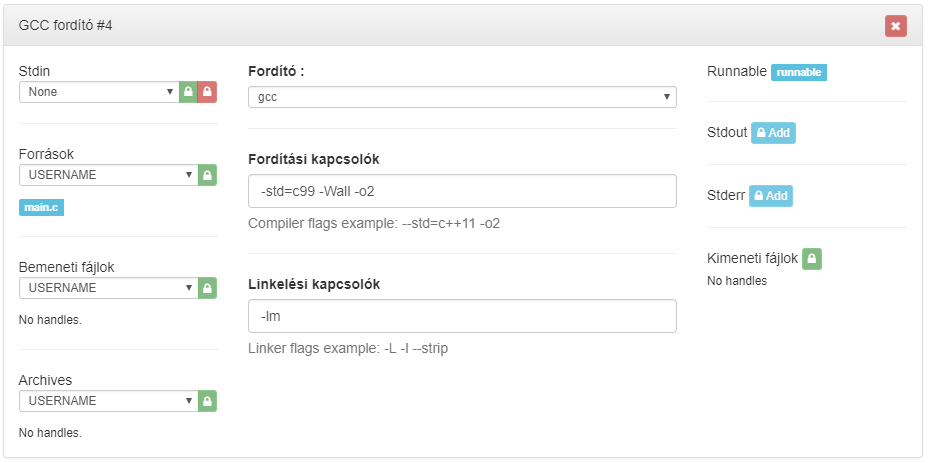
\includegraphics[]{exercise_blokk.png}
    }
    \caption{GCC fordító blokk adminisztrációs felülete}
    \label{fig:exercise_blokk}
\end{figure}

A beadás végső eredménye egy speciális blokk értéke lesz. Ennek a SubmissionResult blokknak egy bemente van, mely ha igaz a beadás sikeresnek tekinthető, ellenkező esetben sikertelen.

A blokkok kiértékelése (hasonlóan \aref{section:dynamic_dependencies}. pontban leírtakhoz) egy függőségi gráf felépítésével kezdődik, melynek kezdőpontja a fentebb említett SubmissionResult blokk. Csak azok a blokkok kerülnek kiértékelésre, amelyek (közvetve vagy közvetlen) függnek ettől a blokktól, hiszen a többi nem befolyásolja a beadás sikerességét.  Itt sem megengedettek a körkörös függőségek, tehát az elkészült gráfnak körmentesnek kell lennie.

\section{Jogosultságkezelés a JPortában}\label{subsection:permissions}

A JPorta által használt Django keretrendszer beépítetten tartalmaz egy egyszerű jogosultság kezelő rendszert. Ez lehetővé teszi különböző jogosultságok hozzárendelését felhasználókhoz, vagy felhasználói csoportokhoz. Minden Django modellhez \cite{DjangoModel} tartozik alapértelmezés szerint három jogosultság, melyeket a keretrendszer automatikusan hoz létre. Ezek a létrehozás (add), módosítás (change) és törlés (delete) jogosultságok. Sok esetben már ezek is elegek lehetnek számunkra, de bármikor létrehozhatunk új jogosultságokat, melyekkel személyre szabottabban tudjuk kezelni a hozzáférést egy-egy funkcióhoz. Ezeknek köszönhetően alapvetően egyszerűen kezelhetjük a jogosultságok kérdését \cite{DjangoAuth}. Fontos megjegyezni, hogy Django-ban a \textit{superuser}-nek jelölt felhasználók automatikusan rendelkeznek minden jogosultsággal.

A JPorta ezen felül egyedi megoldást alkalmaz az egyes objektum példányok elérésének szabályozására, mely az access control list (ACL, \cite{ACL}) technikához hasonló. Az ACL minden objektumhoz rendel egy mátrixot, mely oszlopaiban a személyek (actor), soraiban pedig az egyes műveletek (action) találhatóak. Egy személy akkor hajthat végre egy műveletet, ha a mátrix általa és a művelet által meghatározott cellája igaz értéket tartalmaz.

\Aref{fig:acl}. ábra egy ilyen példát szemléltet: az objektumhoz tartozó hozzáférési mátrix értelmében Bob-nak csak olvasási, Alice-nak pedig olvasási és írási joga van. Emiatt Alice mind az olvasási, mind az írási műveletet sikeresen végrehajthatja, Bob azonban írási műveletet nem hajthat végre.

\begin{figure}[h]
    \centering
    \resizebox{\textwidth}{!}{
        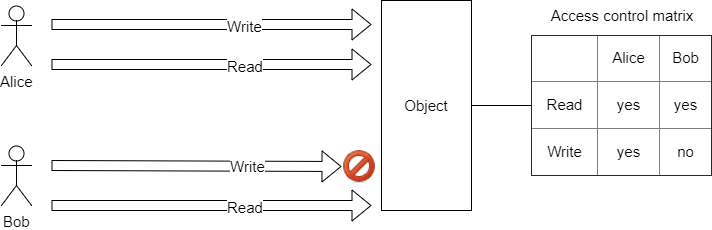
\includegraphics[]{ACL.png}
    }
    \caption{ACL működése és egy hozzáférési mátrix}
    \label{fig:acl}
\end{figure}

A portál közvetlen jogosultságok helyett jogosultsági szinteket használ, tipikusan tulajdonosi (owner) és operátori (operator) szintekkel, de ez modellenként eltérő lehet. Ilyenkor ha egy felhasználót egy objektum tulajdonosának jelölünk, egyben operátori jogosultságokkal is felruházzuk. Ha egy felhasználónak nem kívánunk jogosultságot adni az adott objektumhoz, akkor nem jelöljük egyik szinten sem. Fontos megjegyezni, hogy a \textit{superuser}-nek jelölt felhasználók itt is automatikusan rendelkeznek minden jogosultsági szinttel.

Ez a megoldás kifinomultabbnak mondható az eredeti ACL technikához képest, mivel így különböző műveletek halmazát rendelhetjük egy adott szinthez, pl. az operátor jogosult megtekinteni és módosítani az adott objektum tulajdonságait, de a törléshez már tulajdonosi szintre van szükség.

\section{Jogosultságkezelés felülvizsgálata}

Az automatikus kiértékelő modulnál a jogosultság kezelés korábban nem készült el megfelelően, így ugyan hallgatói oldalról nézve minden jól működött, a feladatokat csak \textit{superuser} jogokkal rendelkező adminisztrátorok hozhatták létre. Ez pedig nagyban megnehezítette felsőbbéves hallgatók, laborvezetők bevonását a rendelkezésre álló feladatok bővítésére. Ennek oka, hogy ekkor minden más adatot is láttak volna a portálon, beleértve minden hallgató eredményeit, megoldásait, ami nem megengedhető.

Ezek értelmében a jogosultság kezelés kibővítésével a cél az volt, hogy egyszerűen és biztonságosan lehessen automatikusan kiértékelődő feladatok létrehozására és szerkesztésére. Az így elkészült rendszer alkalmazza mindkét fenti hozzáférés szabályozási módszert a maximális biztonság és testreszabottság elérésének érdekében.

Ennek elkészítéséhez először a Django jogosultságok ellenőrzését implementáltam, melyhez a beépített \textit{PermissionRequiredMixin} osztályt használtam. Ez egyszerűen teszi lehetővé a jogosultságok meglétének ellenőrzését, csak meg kell adnunk a szükséges jogosultság(ok) listáját, a többit pedig a keretrendszerre bízhatjuk. \cite{DjangoPermissionMixin}

Két jogosultságot használtam fel:

\begin{itemize}
    \item \textit{view\_exercise}: meglétével a felhasználó megtekintheti az összes eddig létrehozott automatikusan kiértékelődő feladatot (exercise). Ennek köszönhetően láthatja, ha már létezik hasonló feladat, mint amire szüksége van, illetve ötletet meríthet a többi feladatból. Emellett pedig a tanulási folyamatot is segíti, hiszen a már meglévő feladatok megértésével fény derülhet az addig rejtélyesnek tűnő működésre.
    \item \textit{create\_exercise}: meglétével a felhasználó létrehozhat új feladatokat. Ilyenkor lehetősége van új, üres feladatot létrehozni vagy egy korábbiról másolatot készíteni.
\end{itemize}

Ezek a jogosultságok fedik le általánosságban a hozzáférések szabályozását. A konkrét feladat példányok hozzáférésének konrtollálásához az előzőek kiegészítésére operátori és tulajdonosi szintet használtam. Ha egy felhasználóhoz egyik sincs hozzárendelve, akkor csak megtekintheti az adott feladatot, nem módosíthatja annak semmilyen elemét. A felhasználói szintek beállítása \aref{fig:exercise_perms}. ábrán látható.

\begin{itemize}
    \item Operátor (operator): az adott feladat példány alap adatait (cím, leírás és címkék), meglévő blokkjait, azok összeköttetéseit tudja módosítani. Lehetősége van más operátor szintű felhasználók felvételére is, illetve egy beadott feladatra újra lefuttatni a kiértékelési folyamatot.
    \item Tulajdonos (owner): az adott feladat példányhoz teljes jogkörrel rendelkezik. Az operátori szint jogain felül hozzáadhat, törölhet blokkokat, más személyeket tulajdonosi szintre emelhet és akár törölheti is a feladatot. Csak tulajdonosok publikálhatnak vagy vonhatnak vissza feladatokat\footnote{A feladat publikálása késznek jelöli azt, melyet csak ilyen állapotban lehet kurzushoz rendelni.}.
\end{itemize}

\begin{figure}[h]
    \centering
    \resizebox{\textwidth}{!}{
        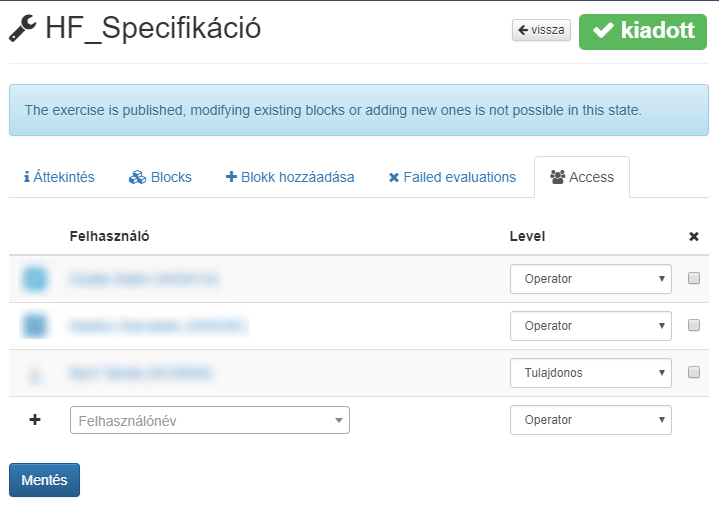
\includegraphics[]{exercise_perms.png}
    }
    \caption{Feladat példányhoz tartozó jogosultsági szintek beállítása}
    \label{fig:exercise_perms}
\end{figure}

Végezetül a szerzői fájlok (ld. \aref{chapter:exercise}. fejezet) hozzáférését ellenőriztem. Itt van lehetőségünk a hallgatók elől elrejteni az adott fájlt, ugyanakkor ez csak a feladatbeadásnál való listázottságát módosítja csak. A fájlok webcím alapján közvetlenül továbbra is elérhetőek maradtak, így próbálgatással az összes titkosnak hitt szerzői fájl tartalmát le lehetett kérdezni. Ennek megoldása egyszerűnek bizonyult, csak módosítani kellett a kérést kezelő függvényben a felhasználó és a visszaadandó fájl ellenőrzését. Eddig a fájl titkos voltától függetlenül visszaadásra került a tartalom.

\section{Kódlefedettség ellenőrzés}

A JPorta elődje révén felmerült az igény a C++ projektek esetében a kódlefedettség ellenőrzésére is. A rendszer bővíthető felépítettsége miatt a kiegészítés a meglévő blokkok és struktúrák lényeges módosítása nélkül lehetséges. Ennek implementálása az alábbi lépéseket foglalta magában:

\begin{enumerate}
    \item Különféle lefedettség ellenőrzők vizsgálata, a megfelelő kiválasztása.
    \item Szükséges Django modellek módosításainak tervezése és implementálása.
    \item Feladat blokk tervezése és implementálása az adminisztrációs felületre.
    \item Kapott nyers adatok feldolgozása.
    \item Felhasználó (hallgató) számára megjelenítés elkészítése.
\end{enumerate}

Megvizsgáltam különböző C++ programozási nyelvet támogató kódlefedettség ellenőrző eszközöket, melyek közül a \textit{gcov} program használata mellett döntötem. Ennek kimenete kiegészíti a forráskódot azzal, hogy mely sorai hányszor kerültek futtatásra. Minden sor elején szerepel, hogy hányszor futott le. Ezt egy kettőspont követi, majd a sor száma az eredeti forrásfájlt szerint, végül pedig a hozzá tartozó kód. Ha az adott sor nem futott le a tesztesetek során, akkor az elején szám helyett \textit{\#\#\#\#\#} vagy \textit{=====} szerepel. Ennek futtatásához szükséges egyfelől a fordításkor megfelelő kapcsoló átadása, illetve a fordításkor és futtattáskor keletkezett \textit{gcno} és \textit{gcda} fájlok továbbítása a \textit{gcov} számára. Tehát a keletkezett fájl formátuma az alábbihoz hasonló:

\begin{lstlisting}
    -:    1:#include <iostream>
    -:    2:
#####:    3:void do_not_run_me()
    -:    4:{
#####:    5:    std::cout << "do_not_run_me" << std::endl;
#####:    6:}
    -:    7:
    1:    8:void run_me()
    -:    9:{	 
    1:   10:    std::cout << "do_not_run_me" << std::endl;
    1:   11:}
    -:   12:	 
    1:   13:int main()	 
    1:   14:{	 
    1:   15:    run_me();
    1:   16:}
\end{lstlisting}

Az elkészült blokk bemenetei a fordítási egységenként keletkezett \textit{gcno} és \textit{gcda} fájlok és a forrásfájlok. Beállítási lehetőségként szerepel a minimálisan elfogadott lefedettségi érték, mely alatt a beadás sikertelennek bizonyul. 
Ezután elkészítettem a szükséges adminisztrátori felületet a blokkhoz (ld. \ref{fig:jporta_codecov_block}. ábra). Ennek bal oldali oszlopában találhatóak a bemenetek bekötésére szolgáló vezérlők (melyek más blokkok kimenetei), középen a blokk tulajdonságainak beállítása, végül jobb oldalon a kimenet definiálása, mely más blokk bemenetére köthető.
    
\begin{figure}[h]
    \centering
    \resizebox{\textwidth}{!}{
        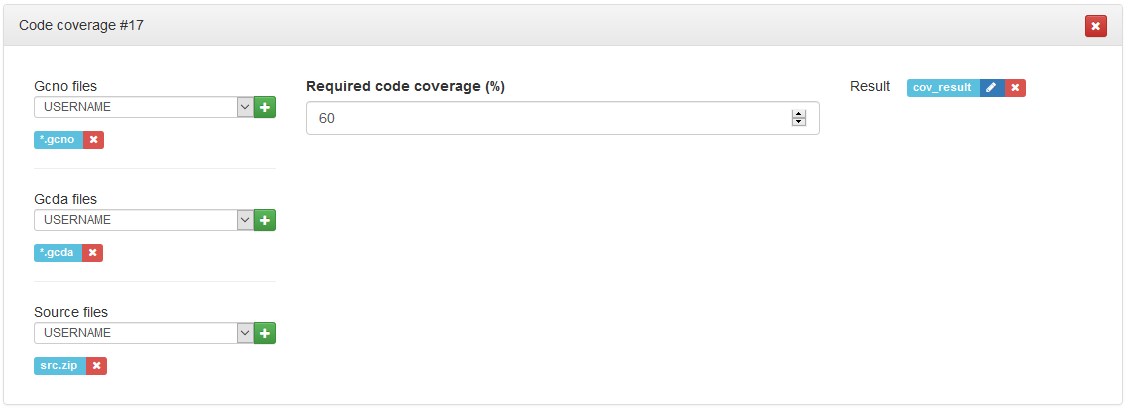
\includegraphics[]{jporta_codecov_block.png}
    }
    \caption{Kódlefedettség ellenőrző blokk}
    \label{fig:jporta_codecov_block}
\end{figure} 

A nyers adatok feldolgozását a modell osztály valósítja meg. Ez a szöveget a megadott formátum szerint elemzi, majd elkészíti a megjelenítéshez szükséges adatstruktúrát.

Végül elkészítettem a hallgatói felületen látható grafikus megjelenítéts (ld. \ref{fig:jporta_codecov_result1}. és \ref{fig:jporta_codecov_result2}. ábra). Itt a hallgató fájlokra bontba megtekintheti, mely sorokat érintette legalább egyszer a tesztesetek során (ezek zöld háttérrel vannak jelölve), illetve azokat, amelyeket egyszer sem (ezek piros háttérrel). A nem színezett sorokban nem található végrehajtható kód. Emellett megtalálható a fájlonkénti és az összesített kódlefedettség is százalékos formában.

\begin{figure}[h]
    \centering
    \resizebox{\textwidth}{!}{
        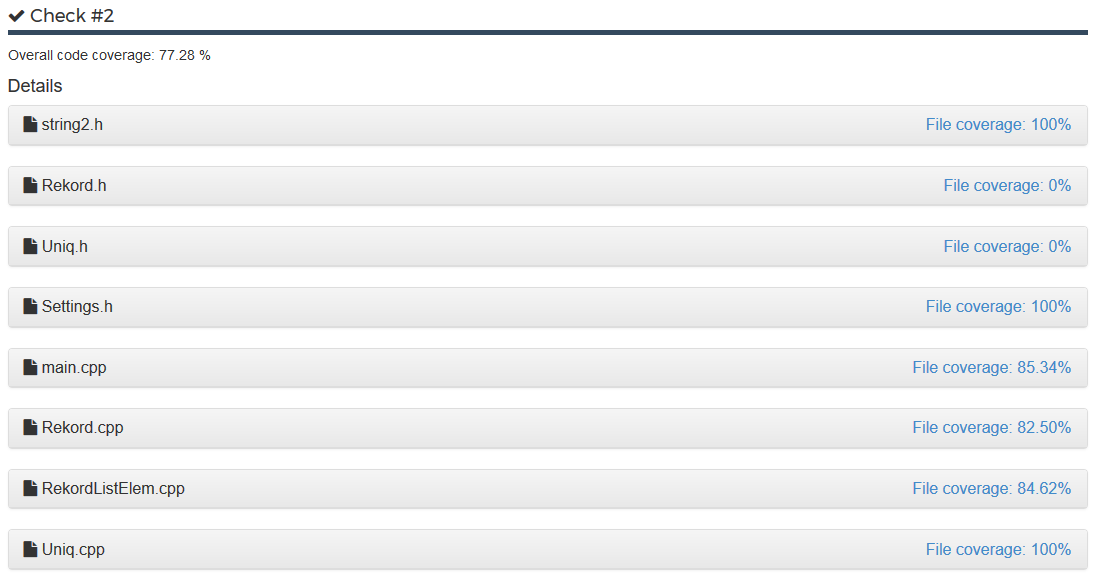
\includegraphics[]{jporta_codecov_result1.png}
    }
    \caption{Lefedettség ellenőrző hallgatói oldalról}
    \label{fig:jporta_codecov_result1}
\end{figure} 

\begin{figure}[h]
    \centering
    \resizebox{\textwidth}{!}{
        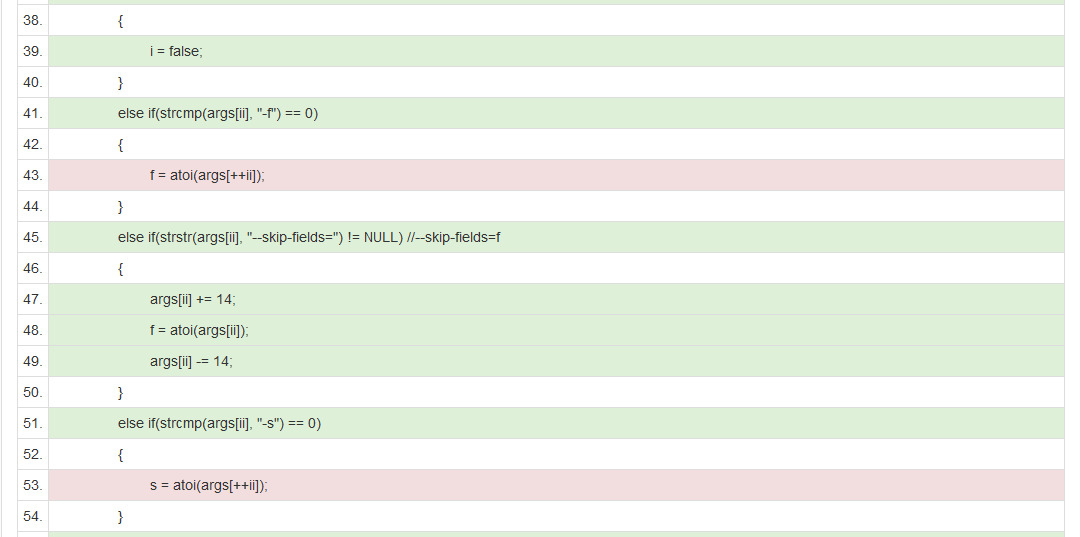
\includegraphics[]{jporta_codecov_result2.png}
    }
    \caption{Lefedettség ellenőrző hallgatói oldalról}
    \label{fig:jporta_codecov_result2}
\end{figure} 

% \section{Feladatok (tesztek) importálása és exportálása}

% \section{Feladatok csoportosítása}

\section{Továbbfejlesztési lehetőségek}

\subsection{Plágiumkeresés}

A portálon beadott megoldásoknak csak akkor van a tanulás szempontjából vett értéke, ha azokat az adott hallgató meg nem engedett segédeszközök nélkül, önállóan oldotta meg. Internetes beadások lévén ennek teljeskörű ellenőrzése önmagában is nehezen vagy egyáltalán nem megoldható feladat. 

Elégséges megoldásként célszerű lenne implementálni egy plágium\footnote{Plágium: ``szellemi tolvajlás, más művének közlése saját név alatt, a mű alapgondolatának vagy részleteinek felhasználása a szerzőre való hivatkozás nélkül'' (Magyar Értelmező Szótár)} ellenőrző blokkot. Itt a blokk bemenete lehet a beadáshoz tartozó forrásfájlok összessége, fő paramétere egy százalékos érték, melyet meghaladó hasonlóság esetén a beadást plágiumgyanúsnak jelöljük, kimenete pedig azon beadások halmaza, amelyekhez az adott forrásfájlok hasonlóságot mutattak.

Írott szövegnél történő plagizálás felderítésénél is felmerül az átfogalmazás problémája. Azaz hogyan detektáljuk, ha a plagizáló nem szó szerint vett át adott részeket, hanem módosítva, de jelentésüket mégis megtartva. Programozási feladatok esetében is felmerül ez a probléma, hiszen sokféle olyan módosítást eszközölhetünk az eredeti forrásfájlon (annak részletes megértése nélkül), mely így látszólag már különbözik. Erre néhány példa lehet a változók, osztályok, struktúrák átnevezése, sorrendjük megváltoztatása, kommentek elhelyezése vagy törlése a kódból, stb.

A plágium detektálást nehezítő faktorok miatt felmerül más szolgáltatások használata is erre a célra. Ilyen szolgáltatás többek között az amerikai Stanford egyetemen készült Moss (Measure Of Software Similarity, \cite{Moss}) szoftver is, mely képes a feltöltöt forráskódok között elvégezni az összehasonlítást. Jelenleg többek között támogatott programozási nyelvek a C, C++, Java, JavaScript, C\#, Python, így tehát az oktatásban használt nyelvek túlnyomó többsége.

Másik problémaként felmerül, hogy a hallgatók nem csak egymás beadásaiból másolhatnak részeket, hanem az interneten keringő egyre több nyílt forráskódú program bármelyikéből. Ezek felismeréséhez számos további probléma megoldására lenne szükség.

\subsection{Verziókezelő támogatás}

Legyen egy projekt akár egyéni vagy csapatos, hobbi vagy megrendelésre készülő, valamilyen verziókezelő rendszert célszerű használni. Ennek fő előnye, hogy folyamatosan nyomon tudjuk követni a projekt változásait, ha pedig azt látjuk a fejlesztés rossz irányt vett, bármikor visszatérhetünk egy korábbi verzióra és folytathatjuk onnan a fejlesztést. Emellett legtöbb ilyen szoftvernél lehetőségünk van több ágon is folytatni a fejlesztést, aminek köszönhetően egyszerűen adhatunk ki hibajavítást egy korábbi verzióhoz, ha szükséges.

Programozóként elkerülhetetlen verziókezelő rendszerekkel való találkozás, ezért az egyetemi oktatásban is egyre nagyobb szerepet kapnak. Ezt követve lehetne valamely verziókezelő rendszert integrálni a JPorta feladatbeadó rendszerébe, így a hallgatók az adott rendszeren keresztül adhatnának be feladatokat, nem közvetlen a portálra feltöltve.

Ennek előfeltétele, hogy a verziókezelő rendszer képes legyen értesíteni a portált, ha új kód kerül beküldésre, illetve hogy a portál le tudja kérdezni a szükséges fájlokat. Ez a módszer segítene megismertetni a verziókezelők előnyeit a hallgatókkal, akik az ismereteket gyakorlatban sajátíthatnák el. Későbbi feladataik során pedig már ismert technológiákkal kerülnének szembe.